\chapter{Discussion}
I believe that the results in the \CP chapter would not be possible or significantly reduced if we ignored the temporal component of the neural population activity. Even when single unit activity is available, the way neural activity is usually represented is as an average spike rate during the stimuli playback. This seems incredibly naive and disregards a huge amount of the information that has been recorded, especially when considering the existence of neurons that fire a single time with millisecond precision in response to songs that are seconds to minutes long as shown in figure \ref{fig:sparse}. In this light, the absurdity of trying to estimate the discriminability of neural representations of auditory stimuli using estimates of blood-flow that change hundreds of milliseconds after the metabolic activity of hundreds or thousands of neurons change becomes painfully apparent. I suspect that evidence for the neural correlates of \CP exists in population activity much earlier in the ventral auditory pathway than is measurable using techniques such as fMRI.

\begin{figure}[tbp] 
  \centering
  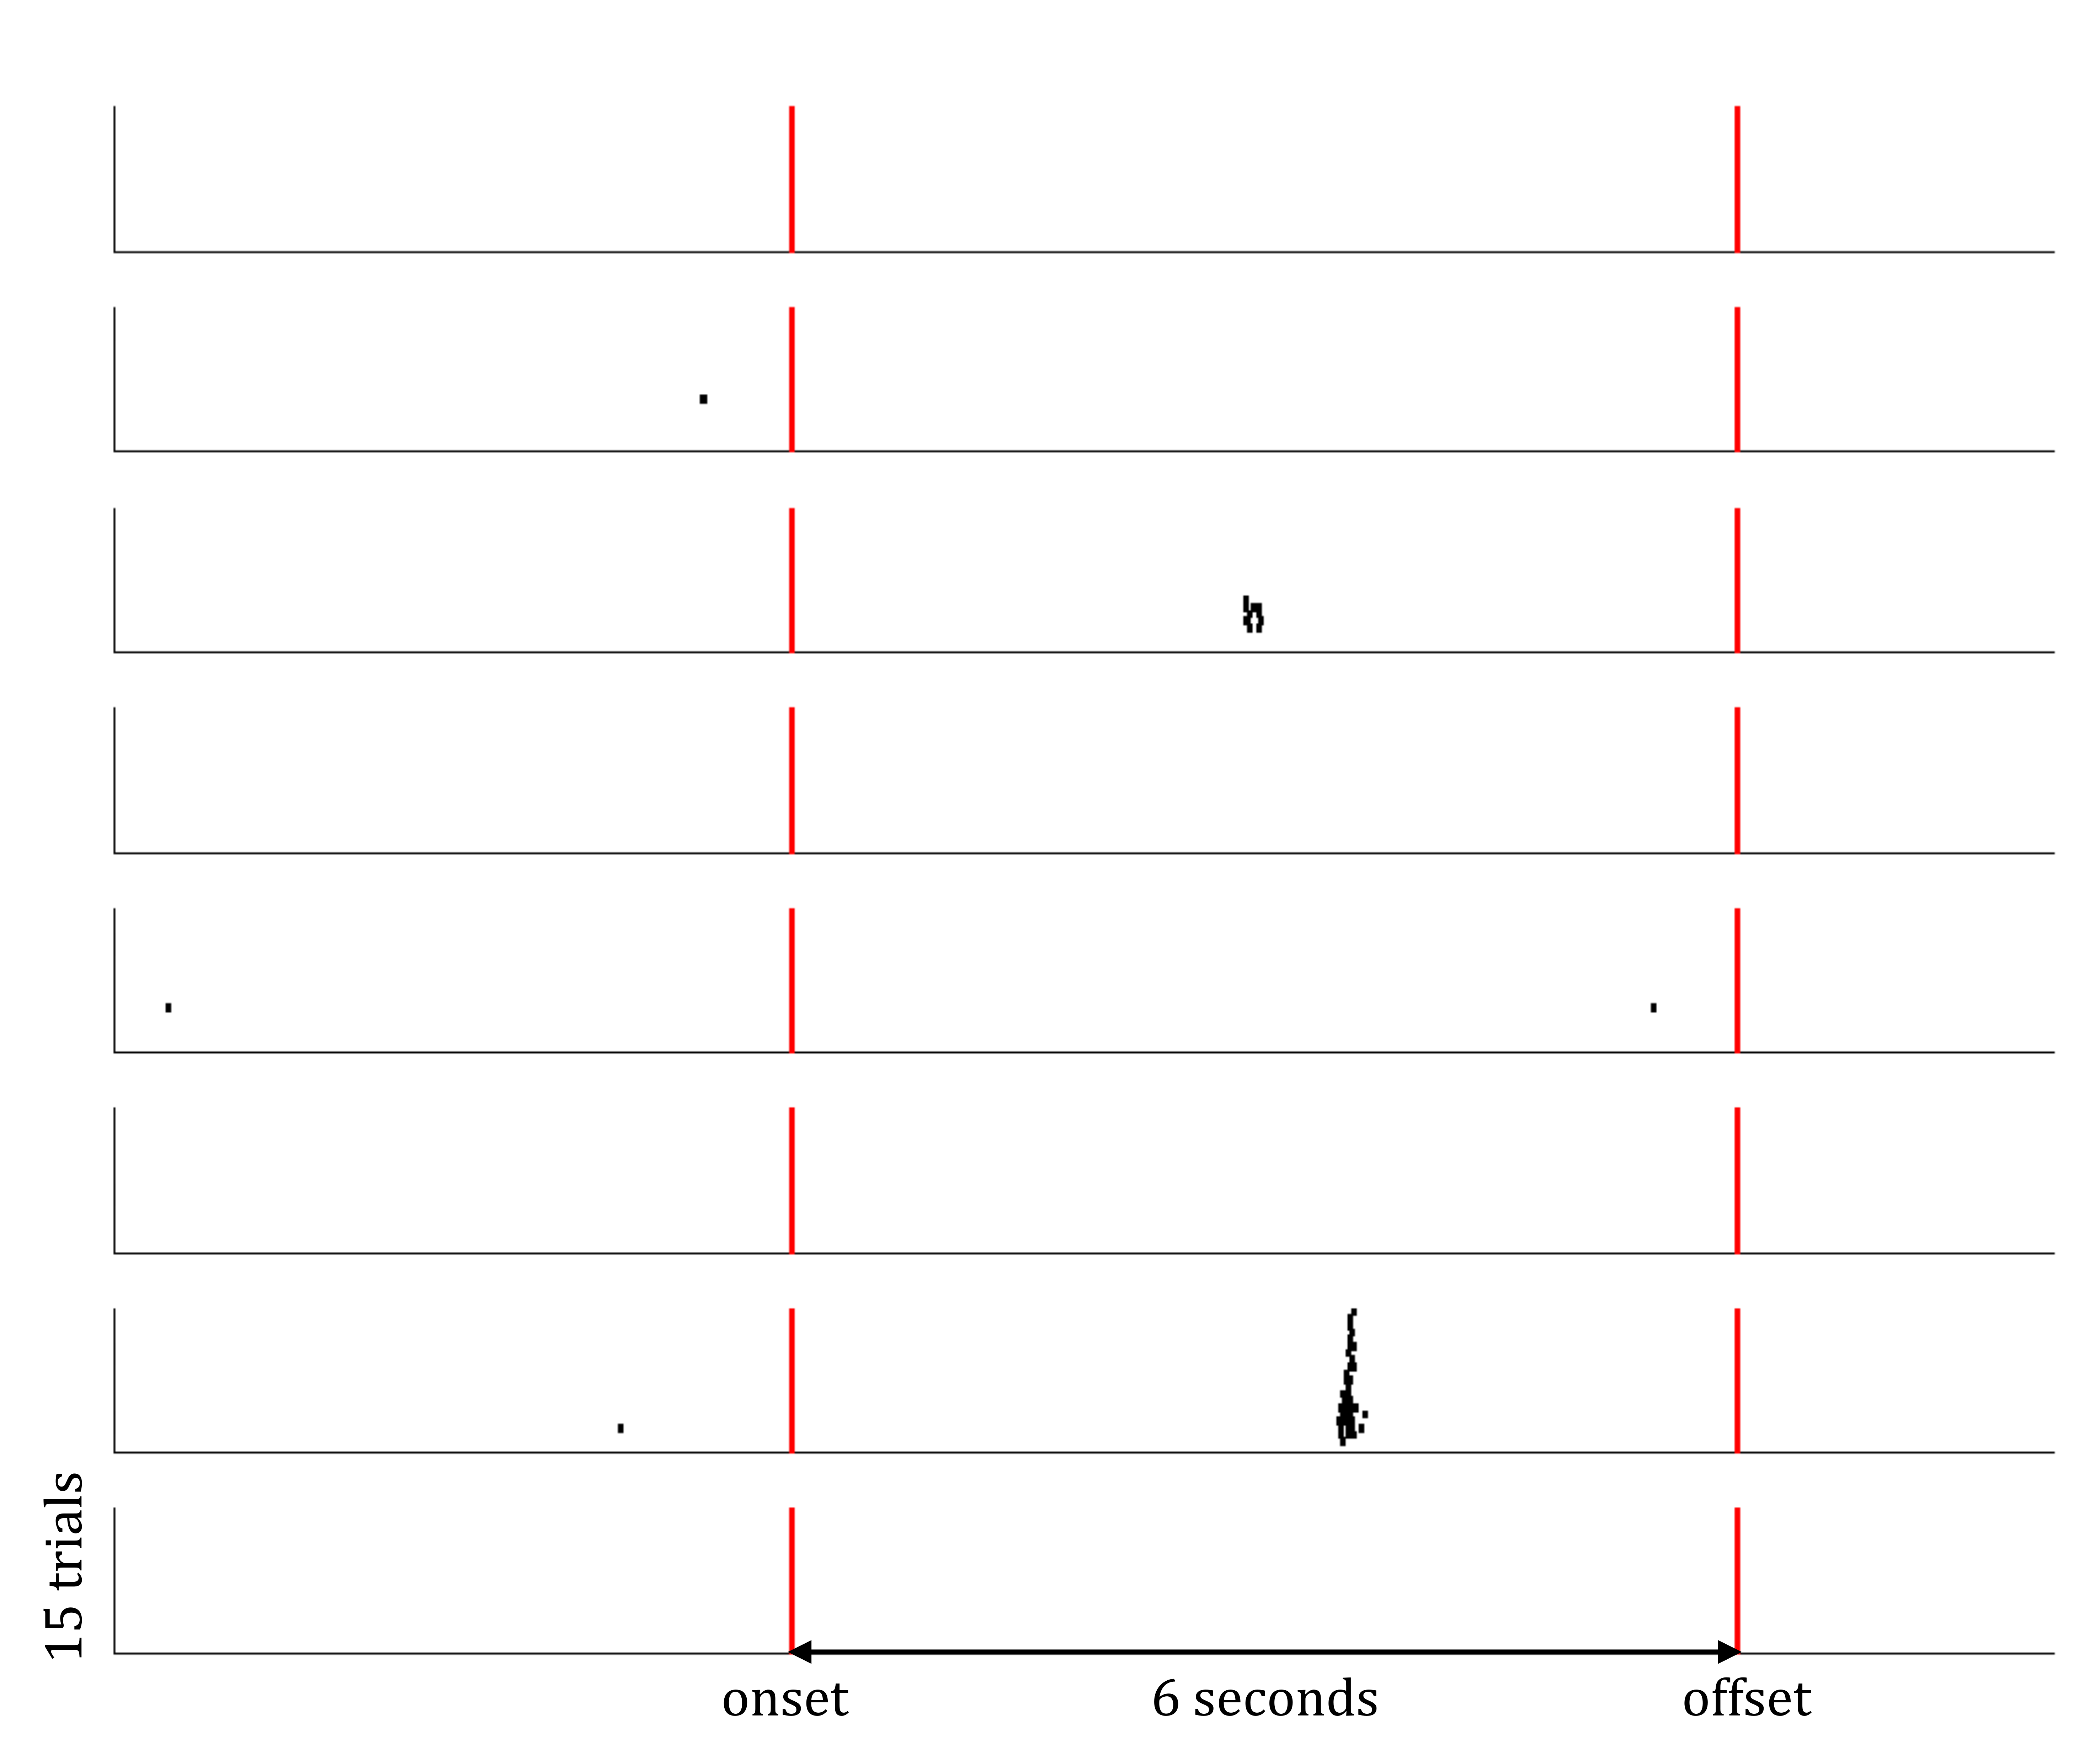
\includegraphics[width=.9\textwidth]{figures/sparse.png}
  \caption[Sparse firing of NCM neuron.]
{The sparseness of firing by an intracellularly recorded neuron from NCM, a secondary auditory region recorded by Dr. Krista Perks. A raster plot of 8 different 6 second long songs, which were presented to this neuron 15 times each. Each vertical black tick represents a single spike. Stimuli onset and offset are plotted in red.
\index{sparse}}
  \label{fig:sparse}
\end{figure}

It seems likely that in our experiment, the birds did not have to shift their representations, but instead just used preexisting features to classify the stimuli. Similarly, human languages may have adapted to use phenome boundaries located in regions with preexisting features allowing for easier discrimination\cite{kuhl1975speech,stevens1981constraints}.

Overall, I believe these methods represent a new potential direction for research into \CP and representations in secondary perceptual regions.

A similar method to the \Thielk curve analysis could also be applied to the exploration of artificial neural network representations. A separate generative technique could be used to probe category boundaries in a machine learning model trained in a supervised manner on categories. This may be a more effective way to explore how different morph interpolation techniques affect the curves. It has been shown that stimulus naturalness could be a factor in determining the degree of categorical perception\cite{van1999categorical} so it would be interesting to see how stimulus naturalness would affect the \Thielk curve. Since there is a remarkable improvement in the state of the art generative models\cite{GAIA, van2016wavenet, waveglow} far beyond the techniques it was originally measured on it would be interesting to see if the \Thielk curve shows a similar function of stimulus quality or if the recent advances have hit the ceiling of the effect.

\section{Analysis Motifs to learn from}
This thesis represents my attempts to apply machine learning and develop techniques to handle high dimensional temporal data in neuroscience. As neuroscientific data acquisition techniques have advanced, we now record more data than was previously imaginable. Our attempts to interpret these data in some way parallel the evolutionary forces that drove the brain to process and interpret the many high dimensional sensory signals it receives. In general, there are several analysis motifs that I'd like to incorporate into my repertoire moving forward.

\begin{enumerate}
    \item Representation matters
    \item Dimensionality matters
    \item Don't throw out temporal information
    \item Don't assume linear scaling
    \item Don't assume normal distributions
\end{enumerate}

\subsection{Representation matters}
When I started my Ph.D. in 2012, the AI winter was ending, and machine learning was regaining commercial acceptance and funding was increasing dramatically. There was much talk about the Universal Approximation Theorem of neural networks \cite{csaji2001approximation} which states that a feed-forward network with a single hidden layer containing a finite number of neurons can approximate continuous functions on compact subsets of $\mathbb{R}^n$, under mild assumptions on the activation function. Crucially, however, it does not touch upon the algorithmic learnability of these parameters. There was a consensus that Deep Neural Networks had completely replaced hand-tuned features and that the best approach was feeding in the raw values and letting the neural networks learn the optimal features. While this does work given infinite data, data has proven to be the limiting factor in all real-world situations\cite{halevy2009unreasonable, sun2017revisiting}. Figure \ref{fig:derivative}K is an example of this. The optimized polynomial coefficients completely determine the evaluated \Thielk curve; however, the predictive power of even XGBoost differs between them. This is a result of a combination of the kernel effect and how disentangled the data is. 

I think a useful metric for the quality of a representation would be the area under the performance curve plotted against the log of the dataset size (scaled by the max performance achieved on the task). This would, of course, be dependent on the task, but it would be a measure of how good a representation is for a given task. The ideal representation (the labels, for example) would take very few samples to reach max performance and would, therefore, have a metric value close to one. This would be especially beneficial for auditory domain questions where many parameters go into the construction of a mel-scaled spectrogram, and I haven't seen too many principled determinations of those parameters.

\subsection{Dimensionality matters}
The curse of dimensionality is real and affects much of the work we do in neuroscience. It refers to the fact that the volume of space increases exponentially as you increase the dimensionality resulting in any available data becoming sparse. Typically downsampling or linear methods such as PCA have been used to reduce the dimensionality, however, with enough data, newer methods such as autoencoder-styled unsupervised techniques can be used as a non-linear analog of the linear techniques. If you have enough data samples to begin to describe non-linear interactions, these techniques can often be a drop-in replacement for the linear techniques. They work by compressing the representation through an information bottleneck, and can often succeed in disentangling the data for an improved representation.

\subsection{Don't throw out temporal information}
This motif was mostly explained in the predictive coding chapter, but in general, there are time components to nearly all of our data and if you ignore time you miss out on a lot of the structure of your data. A movie wouldn't be quite as moving if we collapsed each pixel value across time to form a static image. Even when viewing a static image, our sensory stream consists of a sequence of local perceptions as we move our fovea using saccades which are later integrated into a complete perception. Sequential information is meaningful and important, and we do ourselves a disservice by ignoring it.

\subsection{Don't assume linear scaling}
Very often, the absolute value of a measure is not as meaningful as the order or relationship between elements. Sometimes this can be rectified by explicitly rescaling the data if you have some a priori of how it should be scaled, however, other times it is better to consider the space more as a partially ordered set (poset). This is another reason I like \KS test and the \KS metric, it only requires a partial ordering of the distribution and is invariant to monotonic transformations like taking the square or log of the values.

In the context machine learning and even stochastic gradient descent, an interesting approach would be to train on pairs (or more) of data points to correctly order them and let softmax deal with it in the end. This could allow for more information to be extracted from some metrics that wouldn't necessarily be available if trained only on the labels. Imagine a training set of memes or videos and you want to predict which will go viral. A model that predicts which of two exemplars got more views would likely be able to learn a lot more about what drives virality than a model that simply outputs a probability of a single exemplar going viral.

Another exciting extension of this idea would be to create sorting layers in machine learning. Instead of explicitly taking the max or min of a pool, the output would be all the values in sorted order. Since it doesn't change any values, you wouldn't even have to worry about differentiating the operation, just matching the assignment. This would be very interesting to form a Hero2vec representation for something like a moba. Each hero could be represented as an $N$ dimensional vector representing $N$ unlabeled attributes. The team composition would be represented as a matrix of team members (usually 5) by $N$ attributes with each attribute in sorted order. This would also make the network permutation invariant which could apply to many applications.

\subsection{Don't assume normal distributions}
This is simply an extension of don't assume linear scaling. If you know what the scaling or distribution should be you can perform some transformation; however, there are methods like the \KS test that only assume a partial ordering of the distribution.

\section{Conclusions}
The recent explosion of progress in machine learning provides an opportunity to solve many long-standing as well as many newly emerging problems in the field of neuroscience. I expect machine learning solutions to engineering problems in neuroscience will drive much progress in the field for a long time, and I am glad to have participated in its inception/revival.